% ==============================================================================
% ТЕСТОВЫЙ ФАЙЛ ВЕРИФИКАЦИИ СБОРОЧНОГО КАРКАСА (Фаза B, Задача B01)
% Не входит в основной текст диссертации; служит для проверки чистоты сборки
% ==============================================================================
\documentclass[12pt,a4paper]{report}

% ==============================================================================
% ПРЕАМБУЛА СБОРОЧНОГО КАРКАСА ДИССЕРТАЦИИ (Фаза B, Задача B01)
% Изолированные настройки форматирования, пакетов и служебных макросов
% ==============================================================================

% Кодировки и языковая поддержка
\usepackage[T2A]{fontenc}
\usepackage[utf8]{inputenc}
\usepackage[russian]{babel}

% Математический аппарат
\usepackage{amsmath,amssymb,amsfonts}

% Графика и таблицы
\usepackage{graphicx}
\usepackage{booktabs}
\usepackage{tabularx}
\usepackage{longtable}
\usepackage{multirow}
\usepackage{enumitem}

% Оформление правок и цвета
\usepackage{ulem}
\usepackage{xcolor}

% Поля страницы (базовый стандарт A4 для контрольного переноса)
\usepackage{geometry}
\geometry{top=20mm,bottom=20mm,left=25mm,right=20mm,marginparwidth=18mm}

% Маршруты поиска графических активов:
% 1. figures/ — приоритетный каталог для новых и модифицированных иллюстраций автора;
% 2. extracted/ — каталог базовых медиафайлов baseline v0.5 (исключает дублирование файлов в репозитории).
\graphicspath{
    {figures/}
    {../migration/extracted/DISS-005/50516d7832e6ea133d77b11b48802c4ed1929283ea7601134b878fab0e0338f7/media/}
}

% Гиперссылки и метаданные PDF
\usepackage{hyperref}
\hypersetup{
    colorlinks=true,
    linkcolor=blue,
    citecolor=blue,
    urlcolor=blue,
    pdfauthor={Евдаков А.Е.},
    pdftitle={Диссертация: Исследование и разработка адаптивных алгоритмов БАВР с применением методов машинного обучения}
}

% ------------------------------------------------------------------------------
% Служебные макросы отслеживаемых правок (A07 / revision-policy.md)
% ------------------------------------------------------------------------------
\newcommand{\wordins}[1]{\textcolor{blue}{\underline{#1}}}
\newcommand{\worddel}[1]{\textcolor{red}{\sout{#1}}}
% Чтение B по умолчанию (с сохранением возможности переключения на чтение A)
\newcommand{\wordchoice}[2]{#2}
\DeclareRobustCommand{\wordrevnote}[4]{%
  \footnote{\textbf{Правка [#1]} (#2, #3): #4}%
}

% ------------------------------------------------------------------------------
% Служебные макросы замечаний Word (A05, A06 / DISS-005.json)
% ------------------------------------------------------------------------------
\DeclareRobustCommand{\commentnote}[3]{%
  \footnote{\textbf{Замечание [#1]} (\textit{#2}): #3}%
}

% Исключение служебных макросов из PDF-закладок (outlines)
\pdfstringdefDisableCommands{%
  \def\commentnote#1#2#3{}%
  \def\wordchoice#1#2{#2}%
  \def\wordrevnote#1#2#3#4{}%
}


\begin{document}

\chapter*{Проверка сборочного каркаса}

Данный документ подтверждает работоспособность сборочного каркаса \texttt{manuscript/}:

\section*{1. Проверка кириллицы и типографики}
Проверка русского алфавита: АБВГДЕЁЖЗИЙКЛМНОПРСТУФХЦЧШЩЪЫЬЭЮЯ, абвгдеёжзийклмнопрстуфхцчшщъыьэюя.
Кавычки «ёлочки» и длинное тире~--- работают штатно.

\section*{2. Проверка математического аппарата}
Выключная формула с кириллическим индексом:
\begin{equation}
\label{eq:test_kz}
i(t) = I_{\text{кз}} \cdot \sqrt{2} \cdot \left(\cos\phi_{\text{КЗ}} \cdot e^{-\frac{t}{\tau_0}} - \cos(\omega t + \phi_{\text{КЗ}})\right)
\end{equation}
Ссылка на формулу: \eqref{eq:test_kz}.

\section*{3. Проверка поиска графики через graphicspath}
Загрузка изображения \texttt{image1.png} напрямую из пула извлечённых медиафайлов baseline без дублирования в репозитории:
\begin{figure}[htbp]
\centering
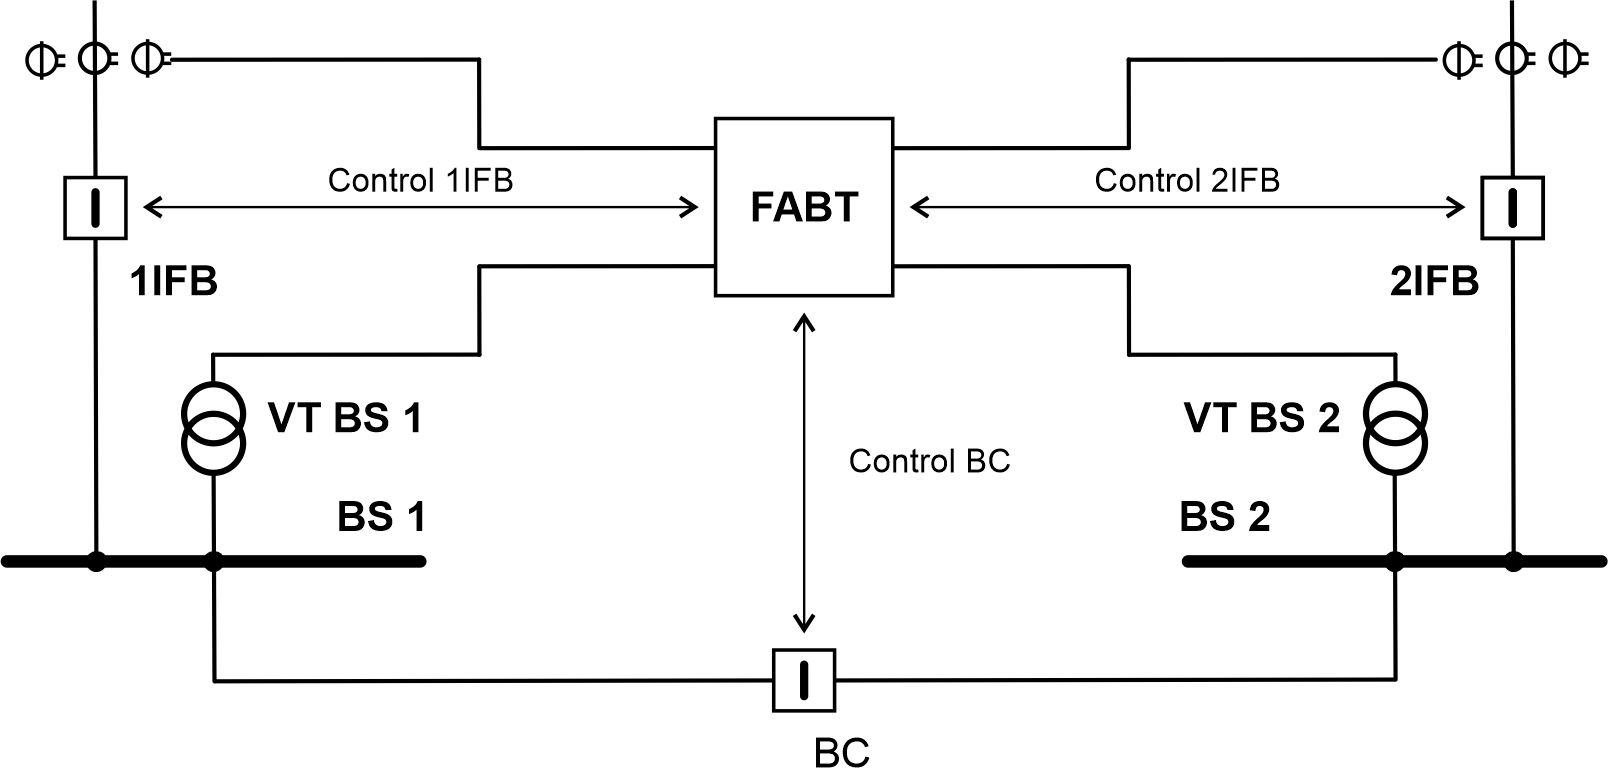
\includegraphics[width=0.45\textwidth]{image1.png}
\caption{Тестовая иллюстрация из пула extracted media}
\label{fig:test_img}
\end{figure}
Ссылка на иллюстрацию: рис.~\ref{fig:test_img}.

\section*{4. Проверка служебных макросов замечаний и правок}
Пример текста с замечанием\commentnote{C0000}{Автор}{Тестовое замечание} и правкой \wordchoice{было}{стало}\wordrevnote{REV0000}{Автор}{2026-09-18}{тестовая правка}.

\end{document}
